\begin{figure*}
\centering
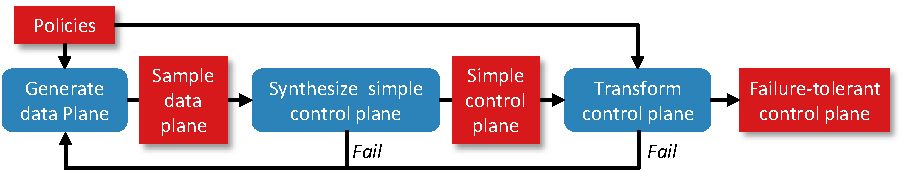
\includegraphics[width=0.7\textwidth]{figures/process.pdf}
\label{fig:process}
\caption{Three-step process for generating a control plane that generates
    policy-compliant paths under bounded failures}
\end{figure*}

\section{Control Plane Synthesis via ARCs} \label{sec:synthesis}
In this section, we describe preliminary ideas on how each phase of our synthesis 
approach can be implemented.
First, we briefly discuss how existing tools can be used to generate
policy-compliant paths (\secref{TODO}).
Second, we show how to generate ARCs that induce
the set of paths synthesized in the first phase (\secref{TODO}).
Third, we show how ARCs can be modified to deal with resilience (\secref{TODO}).
Finally, we show how to restart the process whenever one of the three phases fails (\secref{TODO}).

\subsection{From policies to paths}
The first phase of our approach produces a set of paths adhering to
\loris{what policies}.
Synthesizing sets of paths---i.e., data planes---that adhere to a given set of policies
is already a hard problem, but a few practical approaches have been proposed.
The approach that is most similar to ours is the one used in Merlin~\cite{merlin}.
Given a set of waypoints, reachability, and \loris{traffic load?} policies,
Merlin generates a mixed integer linear programming instance. 
A solution to this instance is a set of paths meeting the input policies.
Our prototype implementation uses a similar idea and,
since this part of the problem is not novel, we briefly provide the intuition behind our solution.
Given a set of policies we generate a set of constraints over the propositional theory of rationals 
and the solutions to these constraints are paths satisfying all the policies that \loris{say which policies
exactly we support at this point}.
Our rich policy language requires complex Boolean reasoning that forces us to adopt propositional theories
in place of simple conjunctions of constraints.
In particular, policies like isolation and waypoints require disjunctive formulas.

%\loris{we will add more details if needed}


\subsection{From paths to ARCs}

The second phase of our approach takes as input the set of paths produced by the first phase
and produces an Abstract Representation of the Control Plane (ARC) that realizes the given set of paths.
First, we  consider the problem of generating ARCs that
 forwards packet bases on shortest-paths---e.g., and ARC representing OSPF routings.
Then, we consider more complex forms of ARCs in which 
 additional mechanisms like route filtering are allowed. 
 
\minisection{From paths to simplified ARCs}
The \emph{Simplified Abstract Representation of the Control Plane} (sARC) is a directed graph comprising switches as 
vertices and weighted edges corresponding to all links in the
topology. 
This is an ideal control plane supporting classic shortest path routing in which no links can be disabled. 

The problem of synthesizing 
a sARC that realizes an input set of paths reduces to a
variation of the so-called {\em inverse shortest path} problem~\cite{}. 
Assume we are given the following inputs: (1) a directed graph $T = (S, L)$ (the network topology), 
(2) a set of endpoints $\Gamma \subseteq S\times S$
describing the sources and destinations of the input paths, and 
(3) a function $P: \Gamma \rightarrow L^*$
that assigns to each pair of endpoints $(s,t) \in \Gamma$ 
an \emph{acyclic} path $P(s,t)=l_0\cdots l_n$ such
that $l_0=(s,s')$, for some $s'\in S$, and $l_n=(s'',t)$, for some $s''\in S$.\footnote{
We use $L^*$ the denote the set of all finite sequences over the set$L$.}
The 
\emph{sARC synthesis}
problem is to find rational weights for the edges in $L$ such that 
for each pair of endpoints $(s,t) \in \Gamma$, 
the path $P(s,t)$ is the shortest path from $s$ to $t$ 
in the graph. 

Since, the forwarding is destination-based,
for a destination $d$, we aggregate the paths 
to create a directed graph $\xi_d$ with the destination
as the sink. Since, the forwarding path cannot have 
loops, $\xi_d$ must be a directed acyclic graph for 
correct enforcement, else we reject the input if this
requirement is not adhered to.
We define $\Omega$ for the 
set of destinations, and $\Delta$ for  
the set of destination DAGs. 
Given $\Omega$ and $\Delta$, we generate a set of linear equations
to find the requisite edge weights of a pure ARC. 
For this, we define $E(sw_1, sw_2)$ as
the edge weight variable for link $sw_1 \rightarrow sw_2$. 
We use $\rightarrow$ operator to denote a path of length 1 
(link), $\rightarrow^*$ to denote a path of length $\geq 0$
and $\rightarrow^+$ to denote a path of length $\geq 1$.
For a path connecting two switches 
$s \rightarrow^+ t$ in a DAG, 
to enforce that the path will be the shortest, we need equations
which ensure the sum of edge weights of the path is strictly smaller than
the weight of all other paths from $s$ to $t$. 

\minisection{Distance Equations}
$D(s,t)$ denotes the absolute shortest distance from $s$ to $t$. 
Trivially, $D(s,s) = 0$. For a path $s \rightarrow^+ t$ ($len \geq 1$),
the shortest distance from $s$ to $t$ is the smallest of the distances
of the paths traversed through the neighbours of $s$ to $t$. The
following equations enforce the semantics of distances; 
here $s \rightarrow sw$ denotes that $sw$ is a neighbour
of $s$, and $sw \rightarrow^* t$ denotes that the path from $sw$ to $t$ contains
zero or more edges.
\begin{multline} \label{eq:dist}
\forall s, t, sw. (s \rightarrow sw \rightarrow^* t).\\
D(s, t) \leq E(s, sw) + D(sw, t)
\end{multline}
Intuitively, $D(s,t)$ is not greater than 
the actual shortest distance from $s$ to $t$.

\minisection{Destination DAG Equations}
For each destination DAG, we add equations to ensure the 
edge weights are set such that a shortest-path forwarding in the ARC 
follows the same path or paths specified in the DAG. If a path
is the shortest path between its endpoints, then every 
subpath of the path has to be the shortest between its endpoints
as well (otherwise the complete path would not be the shortest).
\begin{figure}[h!] 
	\centering
	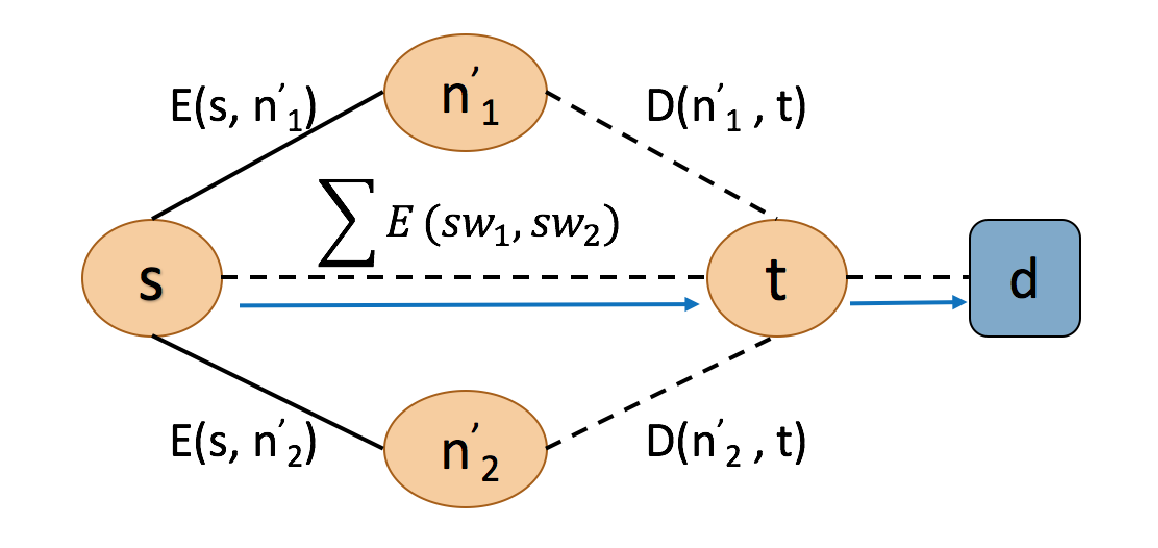
\includegraphics[width=0.8\columnwidth]{figures/distanceEquation.eps}
	\caption{Distance equation} \label{fig:disteq}
\end{figure}
Consider a DAG $\xi_d$ for destination $d$. We define two neighbour
functions: $N(s)$ denotes the set of neighbours of switch $s$ 
in the directed graph, and $N(s, \xi_d)$ denote the set of
neighbours of switch $s$ in the destination DAG. 
Consider a path $s \rightarrow^+ t$ in the DAG ($t$ 
need not be the destination. As the DAG specifies
the shortest paths to the destination, this 
path from $s$ to $t$ has the lowest weight, 
which we express by the sum of weights of 
edges along the path. 
To satisfy the semantics of the ARC,
we need to ensure that all other
paths from $s$ to $t$ are have strictly 
greater path weights.
Thus, we add the following equations to ensure the
shortest path property (\Cref{fig:disteq} illustrates 
an example).
\begin{multline} \label{eq:uniq}
		\forall d \in \Omega. \forall s, t \in \xi_d. (s \rightarrow^+ t).\\ 
		\forall n'. (n' \in N(s) \wedge n' \not\in N(s, \xi_d)). \\
		\sum_{\mathclap{\substack{(sw_1, sw_2) \in (s \rightarrow^+ t)}}} 
		E(sw_1, sw_2) < E(s, n') + D(n', t)
\end{multline}
By using distance for the path $n' \rightarrow t$, we 
are able to find lower bounds to the weight of the non-DAG 
paths from $s$ to $t$,
thus avoiding the blow-up of enumerating all paths from $s$
to $t$. 

% If the path $n' \rightarrow^* t$ 
% is not in any DAG completely, then
% $D(n',t)$ can be smaller than the actual shortest distance by the
% semantics of \Cref{eq:dist} (as
% $D(n',t)$ is not equal to any quantity by \Cref{eq:shortest}).
% However, since $D(n',t)$ is on the RHS of the equations in \Cref{eq:uniq},
% the equations will ensure that the path $s\rightarrow n \rightarrow^* t$
% has strictly greater weight than the path of the DAG.

%TODO: Add some figures
